\section{Swaptions As a Missing Link in Asset Allocation}
When constructing portfolio, there are many considerations and therefore many choice. 
Some of the thing we have to consider is the asset allocation, deriversification, rebalancing 
and risk management. This Section will be a motivation of why it is important to 
allocated to different asset class. The purpose it to see in which market situations
swaption perform better compared to other asset classes.
\\\\
But first a small introduction to portfolio construction. 
So a general  example is a 60/40 weight portfolio, where you allocated 60 percent to equities 
and 40 percent to fixed income. 
The investment belief in most portfolio is long beta, long duration, short volatility and short 
convexity. In other words the portfolio exception is to earn risk premium over the long term, 
where the asset have a long duration, to limited interest rate risk. And you want to be short in
volatility which means that you will sell option to gain risk premium. Secondly we note that we will expected 
a short convexity portfolio to under perform when interest rate are volatile. 
\begin{figure}[H]
    \centering
    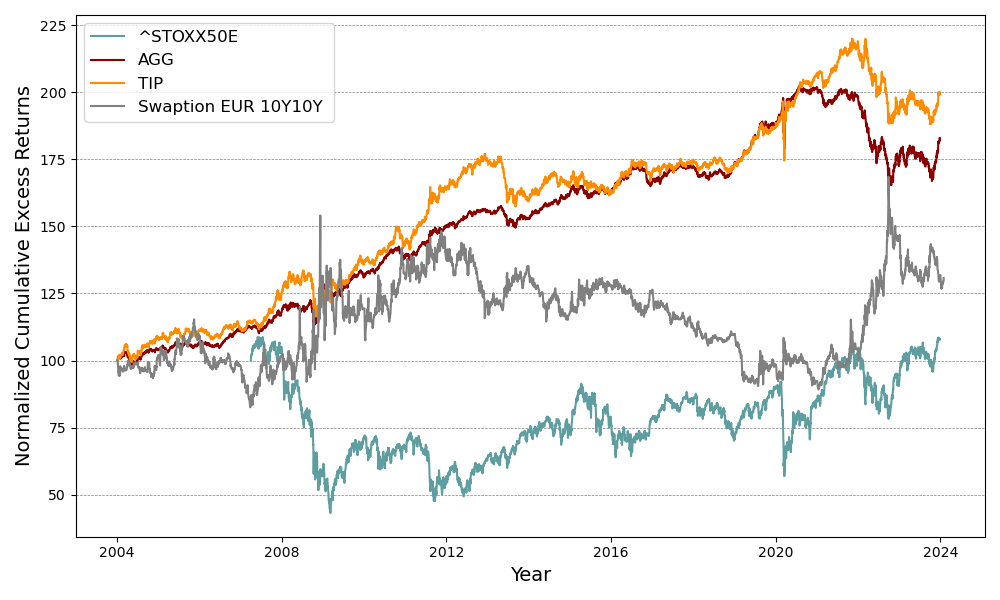
\includegraphics[width=0.9\textwidth]{/Users/nannaingemannohrt/Desktop/master_thesis/main/plots/2004_to_2024_plot.png}
    \caption{Comparison of Normalized Cululative Excess Return. Data source Citi Velocity 21.02.2024 
    and Yahoo Finance.}
    \label{fig:2004_2024}
\end{figure}
\noindent
Moving forward we will look a some market Data from Yahoo Finance and Citi Velocity. 
The purpose is two see how different asset class perform under some particular markets situations.
First a introduction to the different ticker, we will use to illustrated the different asset class. 
We will like to compare perform of the asset class equities, nominal bonds and inflation-linked bonds. 
The performs for the three asset class will be compared to swaption with ten years to expiry and a tenor
of ten years i euro, later in Section \ref{data_lab} the lingo of swaption will be covered. 
Below the chosen ticker are listed, with short explanation. Where the ticker STOXX50E represent equities, 
AGG represent nominal bond and TIP describe inflation-linked bonds.

\begin{itemize}
    \item \textbf{STOXX50E} \text{---}  index of the 50 largest European equities.
    \item \textbf{AGG} \text{---}  index for US investment-grade bond. 
    \item \textbf{TIP} \text{---}  index for inflation-protected US-Treasury secitities.
    \end{itemize}
\noindent
Above in \autoref{fig:2004_2024} the three chosen ticker and the swaption development
is illustrated from 2004 to the start of 2024. Lets start with some general comments.
First of all we note the the same fluctuations appears a cross the thee ticker. 
Secondly we note that these fluctuations does not appears in swaption. 
We might even be abel to see that the opposite fluctuation is represent. 
Then lets remind yourself of some of the most important Finance situations during 
the time period from 2004 to 2024. First but not unnoticed we have the Global Financial Crisis
from 2007 to 2009.  Then we have the COVID-19 Pandemic in 2020 and last recently we have a 
longer period with high inflation starting i 2022. 
\\\\
To underline how swaption perform in this serarinoes, we wee look a the specific time period
around some of the describe situations. Below in \autoref{fig:2007_2011} the same data is illustrated
from 2007 to 2011, this time period includes the Global Financial Crisis 2007 to 2009. 
From this time period we see that equities take a large jump down, where the development of the 
swaption was increasing. So during one of the worst drawdown period in the global market, 
swaption keep performing. In \autoref{fig:2022_2024} we see the data displayed at the 
time period from 2022 to 2024, which is a period with high inflation. 
Here we clearly see the the swaption out perform the other asses class. 
\\\\
This review on some market data, underline that swaption can added some different than some 
of the other asset class. Therefor it could added value to the portfolio constructions. 
But if swaption such take part in the asset allocation, it is important to understand the instrument.
To understand swaption as a instrument, we have to understand all the thing contributing to the price
of a swaption. Then being able to price swaption and analyzing them and manning the risk related to 
swaption.  So moving forward we will start with a introduction to the mathematic of pricing swaption. 
And trough the thesis we will continuing  developing knowledge of swaption and the risk related to swaption.
\begin{figure}[H]
    \centering
    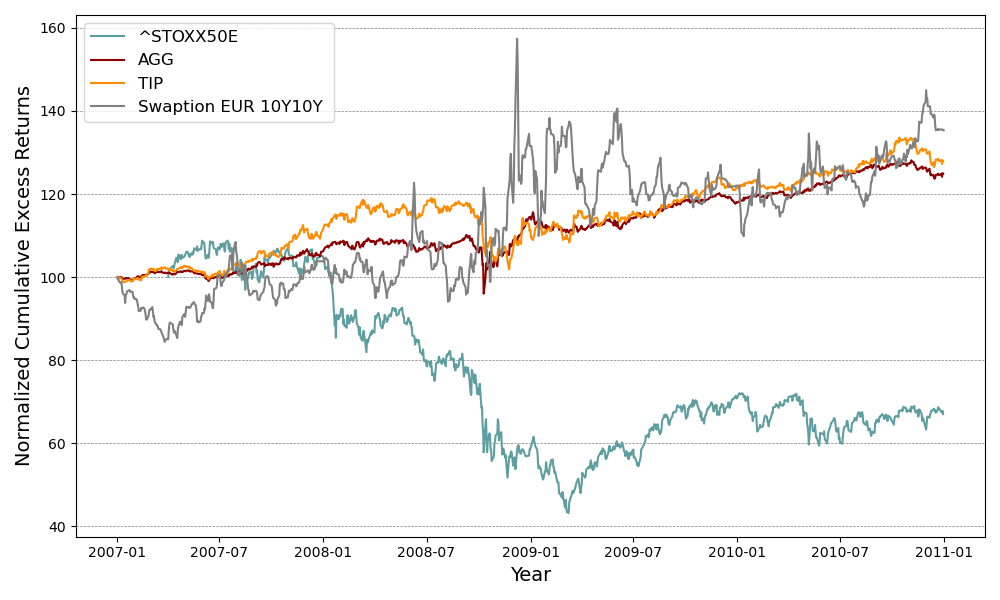
\includegraphics[width=0.9\textwidth]{/Users/nannaingemannohrt/Desktop/master_thesis/main/plots/2007_to_2011.png}
    \caption{Global Financial Crisis 2007 to 2009.  Comparison of Normalized Cululative Excess Return. Data source Citi Velocity 21.02.2024 
    and Yahoo Finance.}
    \label{fig:2007_2011}
\end{figure}
\noindent

\begin{figure}[H]
    \centering
    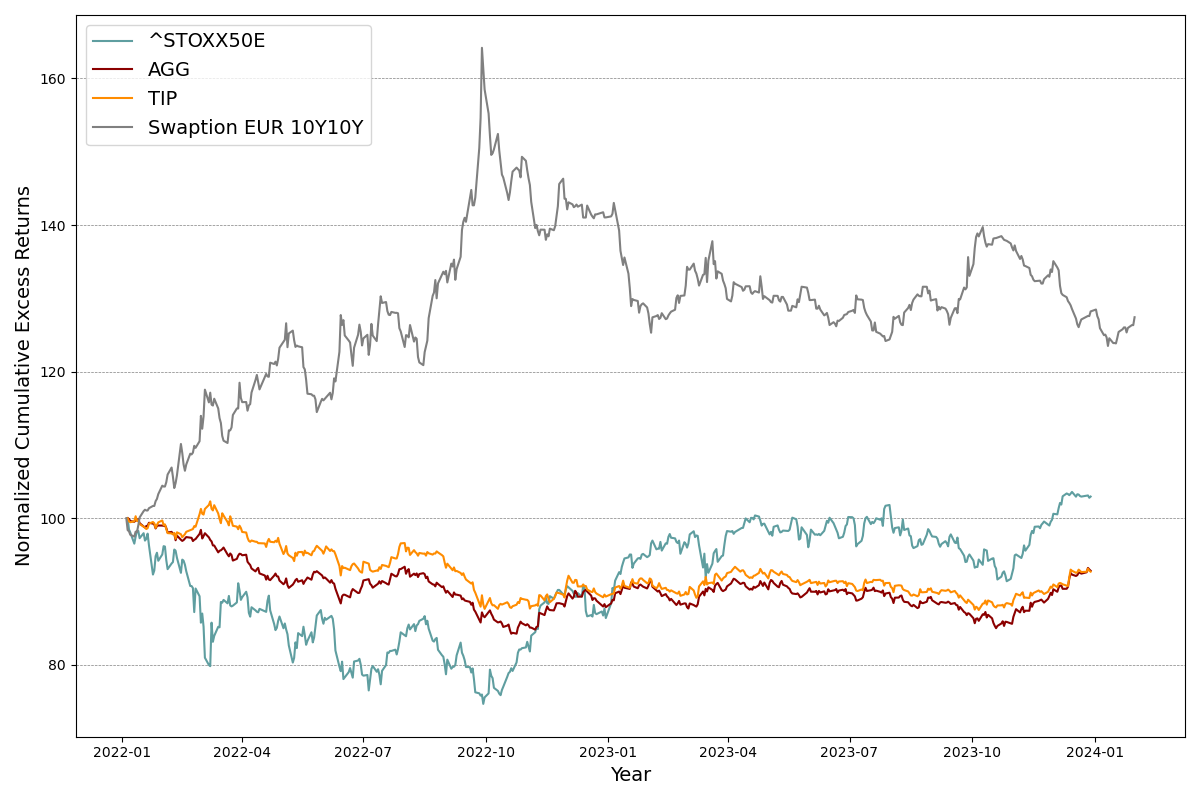
\includegraphics[width=0.9\textwidth]{/Users/nannaingemannohrt/Desktop/master_thesis/main/plots/2022_to_2024.png}
    \caption{High inflation period 2022 to 2024. Comparison of Normalized Cululative Excess Return. Data source Citi Velocity 21.02.2024 
    and Yahoo Finance.}
    \label{fig:2022_2024}
\end{figure}
\noindent

